\documentclass[12pt, a4paper]{article}
\usepackage[top=1.0in, bottom=1.0in, left=0.8in, right=0.8in]{geometry}

\setlength{\parskip}{\baselineskip}%
\setlength{\parindent}{0pt}%
\usepackage{bookmark}
\usepackage[]{graphicx}
\usepackage{enumitem}
\usepackage{amsmath}
\usepackage{relsize}
\usepackage{cprotect}
\usepackage{amsmath, amsfonts}
\usepackage{siunitx}
\usepackage{mathrsfs}
\usepackage{framed}
\usepackage{enumitem}
\usepackage{tikz}
\usepackage{circuitikz}
\usepackage{float}
\usepackage[english]{babel}
\usepackage{blindtext}

\newlist{notes}{enumerate}{1}
\setlist[notes]{label=\textbf{Note:} ,leftmargin=*}

\newlist{hints}{enumerate}{1}
\setlist[hints]{label=\textbf{Hint:} ,leftmargin=*}

\usepackage{xcolor}
\usepackage{color}
\definecolor{com1}{RGB}{125,125,125}
\definecolor{comment}{RGB}{140,115,115}
\definecolor{numbering}{rgb}{0.2,0.2,0.2}
\definecolor{key}{RGB}{0,0,180}
\definecolor{in}{RGB}{0,100,0}
\definecolor{out}{RGB}{100,30,30}
\definecolor{bg}{RGB}{245,245,245}
\definecolor{bgLight}{RGB}{250,250,250}
\definecolor{string}{RGB}{0,150,0}

\usepackage{hyperref}
\hypersetup{
    colorlinks=true,
    linkcolor=blue,
    filecolor=magenta,      
    urlcolor=blue,
}
\urlstyle{same}

\usepackage{listings}

\lstdefinestyle{py_code}{ %
    backgroundcolor=\color{bg},      % choose the background
    basicstyle=\ttfamily\small,		      % fonts
    breakatwhitespace=false,         % automatic breaks at whitespace ?
    breaklines=true,                 % sets automatic line breaking
    captionpos=b,                    % caption-position - bottom
    commentstyle=\itshape\color{comment},    % comment style
    extendedchars=true,              % use non-ASCII
    frame=single,	                   % single frame around the code
    keepspaces=true,                 % keeps spaces in text
    keywordstyle=\bfseries\color{key},% keyword style
    language=Python,                 	  % the language of the code
    morekeywords={Null},       % add more keywords to the set
    numbers=left,                    % line_numbers (none, left, right)
    numbersep=10pt,                  % line_no - code dist
    numberstyle=\footnotesize\color{numbering}, % line_no style
    rulecolor=\color{black},         % frame_color [!always set]
    showspaces=false,                % show spaces everywhere
    showstringspaces=false,          % 
    showtabs=false,                  % 
    stepnumber=1,                    % step b/w two line-no
    stringstyle=\color{string},     % string literal style
    tabsize=2,	                       % sets default tabsize to 2 spaces
    title=\lstname,                  % show the filename
    escapeinside={(*}{*)},			  % escape from style inside (* *)
    xleftmargin=\parindent,
    belowskip=-1.3 \baselineskip,
    aboveskip=1.0 \baselineskip,
    columns=fullflexible,
    xleftmargin=0.15in,
}
\lstnewenvironment{py_code}
{\lstset{style=py_code}}
{}

\lstdefinestyle{psudo}{ %
    backgroundcolor=\color{bgLight},   % choose the background
    basicstyle=\ttfamily\small,		      % fonts
    breakatwhitespace=false,         % automatic breaks at whitespace ?
    breaklines=true,                 % sets automatic line breaking
    captionpos=b,                    % caption-position - bottom
    commentstyle=\itshape\color{com1},          % comment style
    extendedchars=true,              % use non-ASCII
    keepspaces=true,                 % keeps spaces in text
    language=C,                 	  % the language of the code
    morekeywords={type,NULL, True, False},       % add more keywords to the set
    showspaces=false,                % show spaces everywhere
    showstringspaces=false,          % 
    showtabs=false,                  % 
    tabsize=2,	                       % sets default tabsize to 2 spaces
    title=\lstname,                  % show the filename
    escapeinside={(*}{*)},			  % escape from style inside (* *)
    belowskip=-1.8 \baselineskip,
    aboveskip=0.9 \baselineskip,
    columns=fullflexible,
    xleftmargin=0.2in,
    frame=tb,
    framexleftmargin=16pt,
    framextopmargin=6pt,
    framexbottommargin=6pt, 
    framerule=0pt,
}

\lstnewenvironment{psudo}
{\lstset{style=psudo}}
{}

\graphicspath{ ./ }

\title{\textbf{EE2703 : Applied Programming Lab \\ Assignment 10 \\ Linear and Circular Convolution}} 
\author{Chagari Koushal Kumar Reddy \\ EE20B023} % Author name

\date{\today} % Date for the report

\begin{document}		

\maketitle % Insert the title, author and date
\clearpage

\tableofcontents
\clearpage

\section{Aim}
The aim of this assignment is to:
\begin{itemize}
    \item Perform Linear and Circular convolutions of FIR filters
    \item Perfom Linear convolution using circular convolution
    \item Perform auto-correlations on shifted versions of Zadoff-Chu sequence
\end{itemize}
\section{Assignment}
\subsection{Magnitude and Phase response of FIR filter}
The FIR filter coefficients are present in the 'h.csv' file. The data was extracted from the file and by using the \texttt{scipy.signal.freqz} method, I was able to plot the magnitude and phase response of the FIR filter.
\begin{figure}[H]
    \centering
    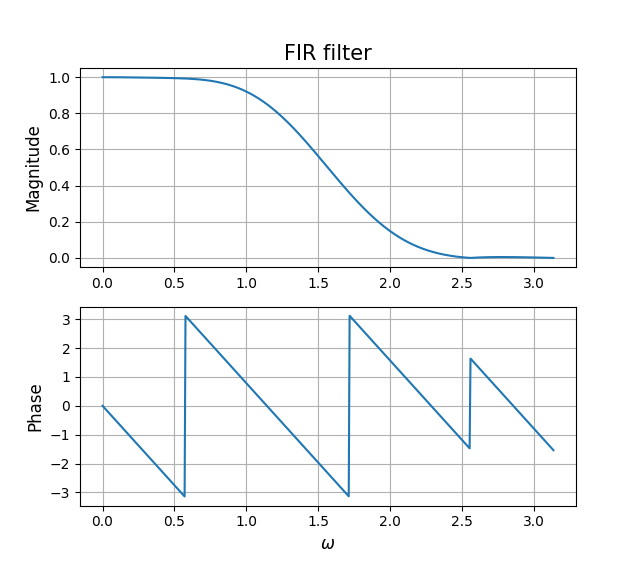
\includegraphics[scale = 0.8]{Figure_1.png}
    \label{fig:sample}
\end{figure}
\begin{center}
    Magnitude response indicates that this is a low pass FIR filter
\end{center}
\subsection{Linear Convolution}
The given signal is $x[n] = \cos(0.2\pi n) + \cos(0.85\pi n)$. The plot of the signal is shown below:
\begin{figure}[H]
    \centering
    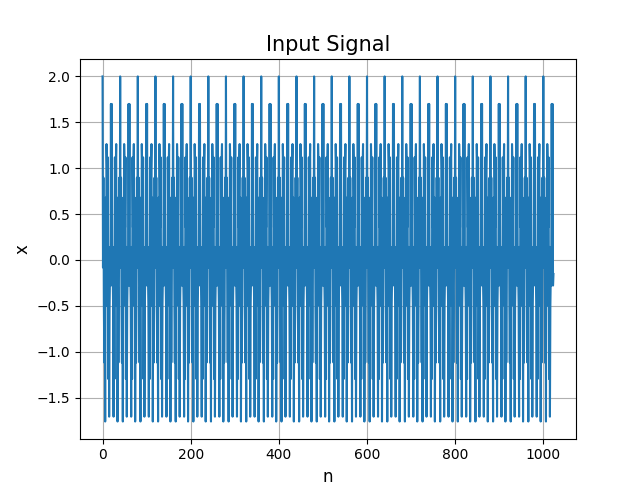
\includegraphics[scale = 0.8]{Figure_2.png}
    \label{fig:sample}
\end{figure}
\begin{figure}[H]
    \centering
    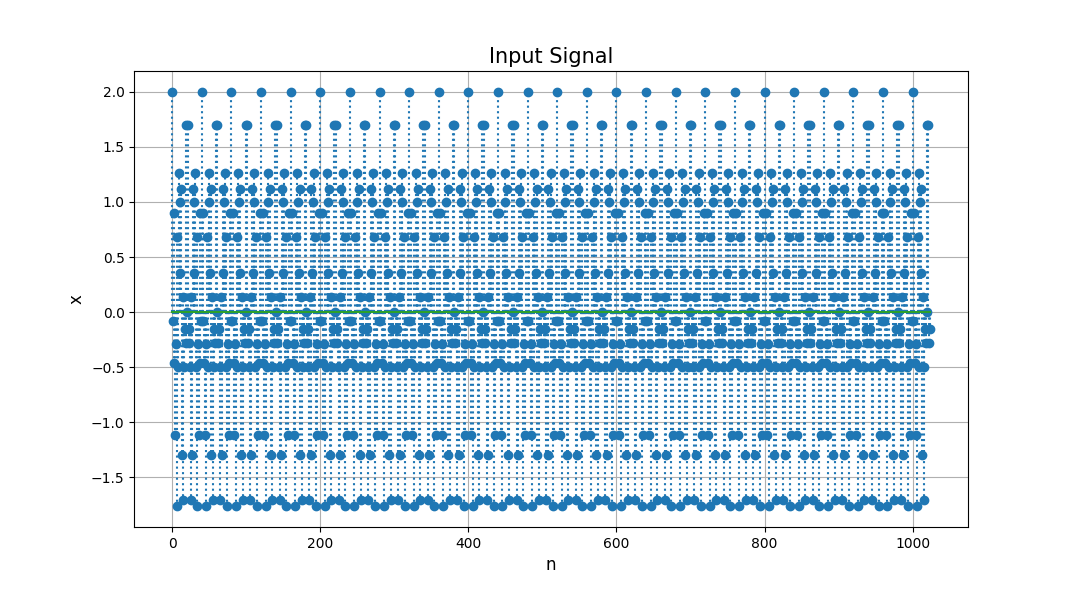
\includegraphics[scale = 0.6]{Figure_2b.png}
    \label{fig:sample}
\end{figure}
This signal is now convolved with the FIR filter using \texttt{np.convolve} which was plotted in the previous section. 
\begin{equation*}
    y[n] = \sum_{k=0}^{N} x[n-k]h[k]
\end{equation*}
The output signal $y[n]$ is shown below:
\begin{figure}[H]
    \centering
    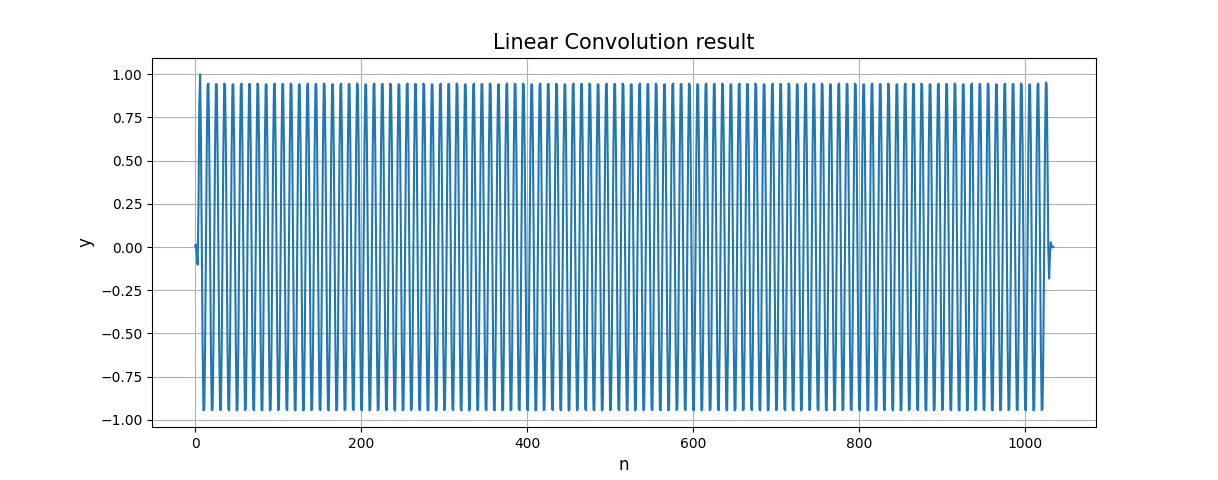
\includegraphics[scale = 0.6]{Figure_3.png}
    \label{fig:sample}
\end{figure}
\begin{figure}[H]
    \centering
    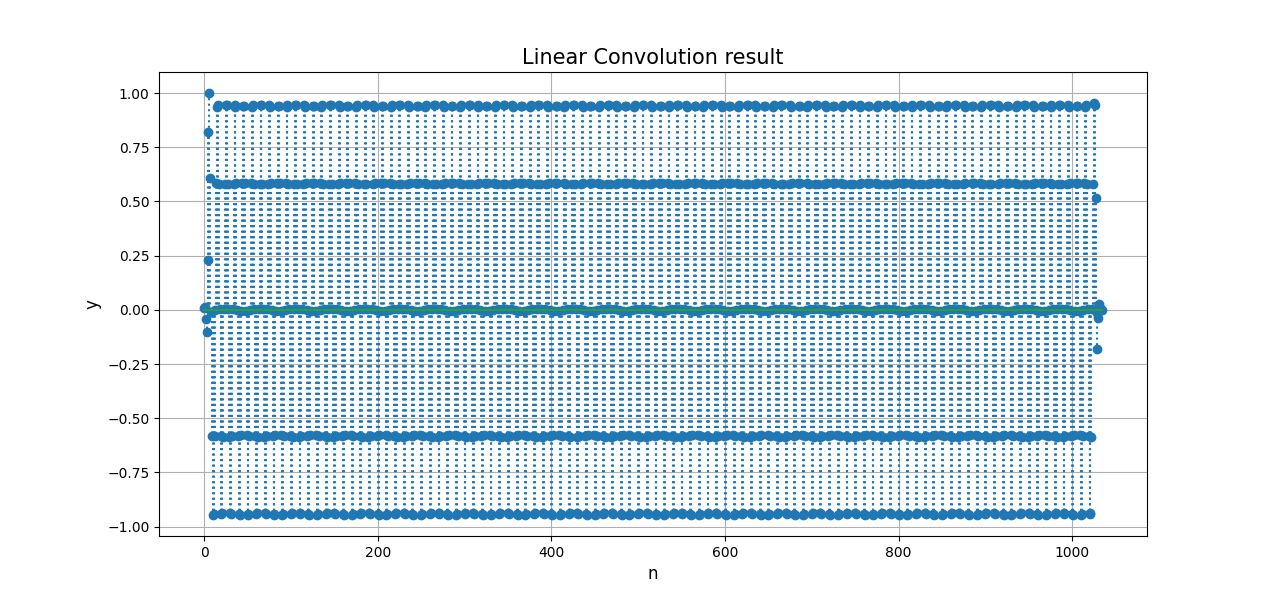
\includegraphics[scale = 0.6]{Figure_3b.png}
    \label{fig:sample}
\end{figure}
\begin{center}
    We can observe that the high frequency component $0.85\pi$ is almost attenuated and the low frequency component $0.2\pi$ is still present
\end{center}
\subsection{Circular Convolution}
\subsection{Circular Convolution as Linear Convolution with Aliasing}

\subsection{Circular Correlation of Zadoff-Chu Sequence}
We now examine the Zadoff-Chu sequence. It has the following properties:
\begin{itemize}
    \item It is a complex sequence
    \item It is a constant amplitude sequence
    \item The correlation of a Zadoff-Chu sequence with a cylically shifted version of itself is 0
    \item  Correlation of Zadoff-Chu sequence with the delayed version of itself will give
    a peak at that delay
\end{itemize}
We will examine the last property of the above list.
\end{document}